\documentclass[tikz]{standalone}
\usepackage{tikz}
\usetikzlibrary{positioning, calc}
\usetikzlibrary{decorations.pathreplacing}
% 定义颜色
\definecolor{color1}{RGB}{144,238,144}  % 浅绿色
\definecolor{color2}{RGB}{173,216,230}  % 浅蓝色
\definecolor{color3}{RGB}{255,255,181}  % 浅黄色
\definecolor{color4}{RGB}{211,211,211}  % 浅灰色
\definecolor{color5}{RGB}{255,182,193}  % 浅粉色

\begin{document}
\sffamily
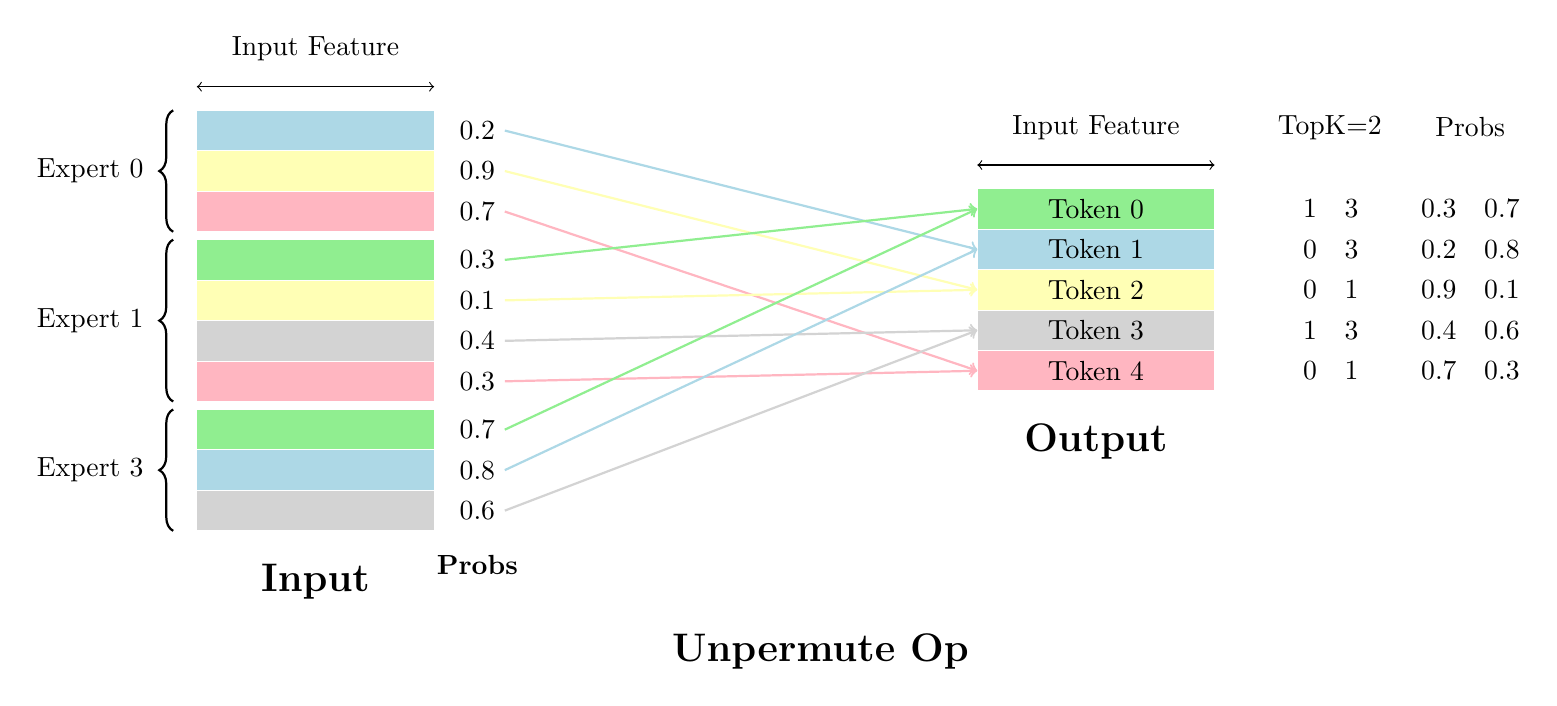
\begin{tikzpicture}[
    token/.style={rectangle, minimum width=3cm, minimum height=0.5cm},
    expert/.style={rectangle, minimum width=3cm, minimum height=2cm},
    output/.style={rectangle, minimum width=0.8cm, minimum height=0.4cm}
]

% 左侧专家输入部分
\node[token, fill=color2] (in0_0) {};
\node[token, fill=color3, below=0.0cm of in0_0] (in0_1) {};
\node[token, fill=color5, below=0.0cm of in0_1] (in0_2) {};

\node[token, fill=color1, below=0.1cm of in0_2] (in1_0) {};
\node[token, fill=color3, below=0.0cm of in1_0] (in1_1) {};
\node[token, fill=color4, below=0.0cm of in1_1] (in1_2) {};
\node[token, fill=color5, below=0.0cm of in1_2] (in1_3) {};

\node[token, fill=color1, below=0.1cm of in1_3] (in3_0) {};
\node[token, fill=color2, below=0.0cm of in3_0] (in3_1) {};
\node[token, fill=color4, below=0.0cm of in3_1] (in3_2) {};

% Input标签
\node[below=0.3cm of in3_2] (input_label) {\Large \textbf{Input}};

% Input Feature标签
\node[above=0.5cm of in0_0] (input_feature_label) {Input Feature};
\draw[<->] ([yshift=0.3cm]in0_0.north west) -- ([yshift=0.3cm]in0_0.north east);

% 大括号
\draw[thick, decorate, decoration={brace, amplitude=5pt}] 
    ([xshift=-0.3cm]in0_2.south west) -- ([xshift=-0.3cm]in0_0.north west) node[midway,xshift=-3em]{Expert 0};
\draw[thick, decorate, decoration={brace, amplitude=5pt}] 
    ([xshift=-0.3cm]in1_3.south west) -- ([xshift=-0.3cm]in1_0.north west) node[midway,xshift=-3em]{Expert 1};
\draw[thick, decorate, decoration={brace, amplitude=5pt}] 
    ([xshift=-0.3cm]in3_2.south west) -- ([xshift=-0.3cm]in3_0.north west) node[midway,xshift=-3em]{Expert 3};


% 左侧概率值
\node[right=0.2cm of in0_0] (probs0) {0.2};
\node[right=0.2cm of in0_1] (probs1) {0.9};
\node[right=0.2cm of in0_2] (probs2) {0.7};

\node[right=0.2cm of in1_0] (probs3) {0.3};
\node[right=0.2cm of in1_1] (probs4) {0.1};
\node[right=0.2cm of in1_2] (probs5) {0.4};
\node[right=0.2cm of in1_3] (probs6) {0.3};

\node[right=0.2cm of in3_0] (probs7) {0.7};
\node[right=0.2cm of in3_1] (probs8) {0.8};
\node[right=0.2cm of in3_2] (probs9) {0.6};

% Probs标签
\node[below=0.2cm of probs9] (left_probs_label) {\bfseries Probs};


% 右侧输出tokens
\node[token, fill=color1, below right=0.5cm and 6cm of probs0] (token0) {Token 0};
\node[token, fill=color2, below=0.0cm of token0] (token1) {Token 1};
\node[token, fill=color3, below=0.0cm of token1] (token2) {Token 2};
\node[token, fill=color4, below=0.0cm of token2] (token3) {Token 3};
\node[token, fill=color5, below=0.0cm of token3] (token4) {Token 4};

% Output标签
\node[below=0.3cm of token4] (output_label) {\Large \textbf{Output}};

% Output Feature标签
\node[above=0.5cm of token0] (output_feature_label) {Input Feature};
\draw[<->] ([yshift=0.3cm]token0.north west) -- ([yshift=0.3cm]token0.north east);

% 中间的概率和编号
\node[right=1cm of output_feature_label] (topk_label) {TopK=2};
\node[right=3cm of output_feature_label] (probs_label) {Probs};

\node[right=1cm of token0] (numbers0) {1\quad{}3};
\node[right=2.5cm of token0] (out_probs0) {0.3\quad{}0.7};

\node[right=1cm of token1] (numbers1) {0\quad{}3};
\node[right=2.5cm of token1] (out_probs1) {0.2\quad{}0.8};

\node[right=1cm of token2] (numbers2) {0\quad{}1};
\node[right=2.5cm of token2] (out_probs2) {0.9\quad{}0.1};

\node[right=1cm of token3] (numbers3) {1\quad{}3};
\node[right=2.5cm of token3] (out_probs3) {0.4\quad{}0.6};

\node[right=1cm of token4] (numbers4) {0\quad{}1};
\node[right=2.5cm of token4] (out_probs4) {0.7\quad{}0.3};


% 连接线,显示概率值
\draw[->, thick, color2] (probs0.east) -- (token1.west); % node[midway,above,font=\small] {0.2};
\draw[->, thick, color3] (probs1.east) -- (token2.west); % node[midway,above,font=\small] {0.9};
\draw[->, thick, color5] (probs2.east) -- (token4.west); % node[midway,above,font=\small] {0.7};
\draw[->, thick, color1] (probs3.east) -- (token0.west); % node[midway,above,font=\small] {0.3};
\draw[->, thick, color3] (probs4.east) -- (token2.west); % node[midway,above,font=\small] {0.1};
\draw[->, thick, color4] (probs5.east) -- (token3.west); % node[midway,above,font=\small] {0.4};
\draw[->, thick, color5] (probs6.east) -- (token4.west); % node[midway,above,font=\small] {0.3};
\draw[->, thick, color1] (probs7.east) -- (token0.west); % node[midway,above,font=\small] {0.3};
\draw[->, thick, color2] (probs8.east) -- (token1.west); % node[midway,above,font=\small] {0.8};
\draw[->, thick, color4] (probs9.east) -- (token3.west); % node[midway,above,font=\small] {0.8};


% Unpermute Op标签
\node[below right=5cm and 2cm of probs2] (unpermute_label) {\Large \textbf{Unpermute Op}};

\end{tikzpicture}
\end{document}